\section{About the dataset}
% TODO: slower introduction into the section, talk about landing fields again
% TODO: elaborate why this specific dataset was used

The dataset which is used throughout this thesis is provided by the Ministry of the Interior of the State of North Rhine-Westphalia in Germany. With the platform GEOportal\footnote{available at \url{https://www.geoportal.nrw/}} they offer various types of maps, like topographical maps, elevation data and orthographical footage. Most of the data is available for free download in batches. The batches used in this thesis are released under the dl-de/zero-2-0 licence. This means that the data can be used for any purpose without any restrictions or conditions\footnote{see the full license text at \url{https://www.govdata.de/dl-de/zero-2-0}}.

For the purpose of this thesis there are two types of maps which prove useful. First, there is a map assembled of digital orthophotos (DOPs). A DOP is an aerial photograph of the surface of the earth. It is processed to hide effects like perspective distortions or topographic features of the landscape. Also it follows a specific map projection to denote the exact spatial extents of the photograph on the earth's surface. Because of that, DOPs are great to analyze terrain coverage and conditions. In section~\ref{sec:segmentation} DOPs are used to perform a semantic segmentation based on the terrain surface.

The second map explored in this thesis contains imagery obtained by near-infrared (NIR) spectroscopy. They are processed in the same way as the DOPs, so they are also projected onto the earth's surface with a specific map projection. NIR data is widely applied in agriculture to monitor the cultivation of herbal products like forages and vegetables. In this thesis the NIR imagery is used to approximate vegetation density for specific regions (see section~\ref{sec:vegetation_analysis}).

\subsection{Getting the dataset}
Both the DOP and NIR datasets are provided by the Ministry of the Interior in a few different ways. To get a quick overview, there is an online viewer for most of the map types available at \url{https://www.tim-online.nrw.de/tim-online2/}. For some specific maps like the DOPs they host a Web Map Tile Service, which allows to access the data with geographic information systems (GIS) like QGIS\footnote{QGIS is a free and open-source GIS application available at \url{https://qgis.org/}}. Since these options require a continuous network connection, it is preferred to get a local copy of the dataset and work with that.

For that purpose, the GEOportal has a separate download section. There you can choose the regions and map types you need and download them in a compressed bundle. The bundle contains map tiles in the JPEG 2000 file format. This is an image format that has a dense compression rate and directly contains the georeferencing for each tile. To have a wide range of terrain types with broad variety included, we use the data for the Municipality of Arnsberg and its surroundings. This concludes to a download size of $11.5~\text{Gigabytes}$ with around $248.49~\text{km}^2$ of terrain, where each pixel represents a $10\times 10~\text{cm}$ square in scale.
% TODO: JPEG 2000 not very widely accepted

It is possible to download both DOP and NIR data together in a single bundle. The JPEG files then contain four bands of pixel information. The first three bands make up the red, green and blue colors for the DOPs. And the last band provides the scalar output of the NIR spectroscopy scan.

% TODO: show some example images from the dataset, maybe later?
% TODO: demonstrate the limits of practical feasibility, maybe later?

\subsection{Preparing the dataset}
As a first step, the whole dataset is imported into a spatial database system. By doing that, it is very easy to export the data in various data formats and tile sizes required by the reference architectures (see section~\ref{sec:ref_archs}). PostgreSQL\footnote{see \url{https://www.postgresql.org/}} is a powerful open-source database system. Together with PostGIS\footnote{see \url{https://postgis.net/}}, a free and open-source extension for PostgreSQL, it is capable of performing spatial operations on image rasters and vector objects. For example, it adds database functions to merge raster tiles, calculate intersection regions or determine bounding boxes.
% TODO: created a database with postgis as single source of truth

The PostGIS installation contains a few shell tools to import data into the database. Unfortunately, they do not support the JPEG 2000 image file format. Before the import of the data can take place, it has to be translated to one of the supported formats first. One of the most widely used formats is GeoTiff. The Tiff file standard is great, because it consists of a baseline section which contains the image information, and a meta section which can contain all kinds of meta information. For example, it can be used to store georeferencing information, which PostGIS is able to use for importing GeoTiff files.

To convert the files from JPEG 2000 to GeoTiff, we use the \emph{Geospatial Data Abstraction Library} (GDAL). This is a tool collection which acts as an abstraction layer for various geospatial data formats. It also includes a shell tool to translate several georeferenced image file formats, including JPEG 2000 and GeoTiff. Listing~\ref{lst:jp2_to_tif} in appendix~\ref{app:code} shows a bash script using the \texttt{gdal\_translate} tool to convert all the JPEG 2000 files to the GeoTiff format.

With the files in GeoTiff format it is now possible to use the \texttt{raster2pgsql} tool to import them into a PostGIS raster table. The whole import process is automated with a Python script (see listing~\ref{lst:tif_to_raster} in appendix~\ref{app:code}). It assumes that there is a database called \texttt{dop10rgbi\_nrw} with the PostGIS extension enabled.

In the first step, the script creates two database tables named \texttt{dop\_rgb} and \texttt{dop\_nir}. The \texttt{dop\_rgb} table has a PostGIS raster column with three raster bands to hold the color information for the DOPs. Simultaneously, the \texttt{dop\_nir} table also has a PostGIS raster column with only one raster band for the NIR values. It is reasonable to separate the color and NIR values as they will be used for different tasks later on.

After the tables are created, the script loops through all the GeoTiff files and calls the \texttt{raster2pgsql} tool for every single one. That call returns some SQL insert statements enriched with the raster information in a binary representation. To execute those statements, it is possible to simply pipe the output of \texttt{raster2pgsql} into a \texttt{psql} command which is connected to the database.

The \texttt{raster2pgsql} tool provides a lot of arguments to properly configure the import of the data. Obviously it needs to know the name of the file to import and the name of the database table to insert the data to. For performance reasons it is very important to set an appropriate tile size for the raster. The original tile size of the GeoTiff files ($10000x10000$ pixels) was assessed to be too large. After some experiments, a tile size of $1000x1000$ pixels was found to work best for both the initial import and the later processing of the raster.

Another major configuration is the spatial reference id (SRID). It also has to be passed as an argument, to ensure the data is imported correctly. The SRID indicates the map projection that is used to map the raster to the earth's surface. The dataset is provided with the SRID 25832. This SRID does not cover the entire globe, but only a rectangular area on the European continent. Therefore it offers a high precision (without too much distortion) in that area and is widely used for maps in Central Europe.

After all GeoTiff files are imported, the Python script creates a Generalized Search Tree (GiST) index for both tables. This takes into account the spatial character of the data and thus speeds up spatial queries (like merging, intersecting) on the tables significantly. For the same reason, the Python script also enforces some constraints on the raster columns of the tables. This makes sure that all the raster tiles share common properties like tile size, SRID or the number of raster bands.

As a last step of the Python script, it creates one last table named \texttt{geom\_bounds}. This table holds a single PostGIS geometry object defining the exact boundaries of the raster tiles. That allows for a quick way to calculate if a given region is included in the spatial extents of the raster without having to process the whole raster table all the time.
% TODO: show some images and explain the dimensions (1px = 1dm)

% TODO: reference figure
\begin{figure}[h]
    \centering
    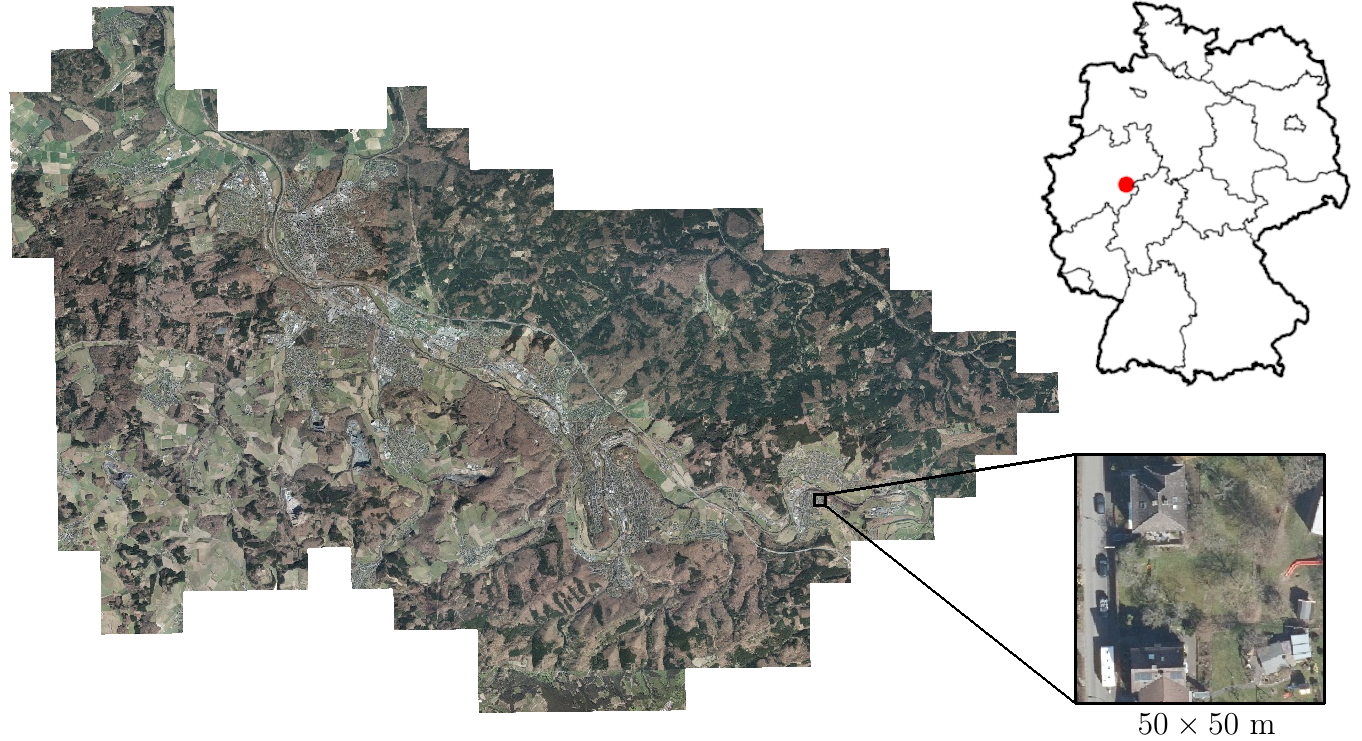
\includegraphics[width=\textwidth]{images/dop_rgb_all}
    \caption{The DOPs in the dataset}
    \label{fig:dop_rgb_all}
\end{figure}

\subsection{Preparing the labels}
As explained in section~\ref{sec:dl_paradigms}, for supervised training you need to provide the model with a pair of input and expected output. The DOPs explained in the previous section function as input for the model. To train the model for segmentation, another prerequisite is to have some segmentation examples prepared. Usually this task is done manually by lining out the segments of a tile and then assigning a category to each segment.

To reduce the amount of work, we use another dataset from the GEOportal called Digital Basic Landscape Model~\cite{base-dlm20}. It describes topological features of the landscape in a vector data format. Besides other things like \WIP{points of interest}, it includes regions categorized by their respective land use. The dataset is available for free download and also permits any use within the dl-de/zero-2-0 license. With some transformation the data fits perfectly for the use as labels during the training of a model.

The categorized regions are provided as Shapefiles. Shapefile is a specific data format for vector-based geospatial objects. To have all data in a single source system, the Shapefiles are imported into the PostGIS database. This also makes it easier to export the segmentation information later on for different tile sizes. Again, the import process is automated with a Python script (see listing~\ref{lst:tif_to_raster} in appendix~\ref{app:code}).

PostGIS includes a tool called \texttt{shp2pgsql} to import Shapefiles into a database table with a PostGIS geometry column. It takes into account all the metadata that is listed in the Shapefile and creates separate columns for those values. The Python script loops over all the required Shapesfiles and calls the \texttt{shp2pgsql} tool passing some arguments like the target SRID. At first, each file is imported in its own database table. This is because each file contains a specific set of meta information resulting in different table layout for each file. The categorized regions are now represented as PostGIS geometry objects.

The original Shapesfiles enclose all regions of the State of North Rhine-Westphalia. Since the DOP und NIR datasets only consist of a smaller subregion, all geometry objects are cropped to that subregion in the next step. Geometry objects that are located outside of the boundaries are dropped entirely. During this process, the tables of the different Shapefiles are merged into one single table. This resulting table has columns for an internal id, the object type, a textual object description and for the geometry object itself. As all the other meta information contained in the Shapefiles is not needed, it is dropped in this step.

The Shapefiles contain a few more categories than the segmentation in this thesis aims for. For example, the difference between industrial zones and housing zones is negligible for the purpose of emergency landings. Thus, the categories are mapped to six predefined supercategories:
\begin{itemize}
  \setlength\itemsep{1mm}
  \item water
  \item buildings
  \item agriculture
  \item forest
  \item urban greens
  \item traffic
\end{itemize}
The mapping between the categories of the Shapefiles and the chosen supercategories is to be found in table~\ref{tab:category_mapping}.

\begin{table}[]
\centering
\small
\caption{Mapping from Shapefile objects to segmentation categories}
\label{tab:category_mapping}
\begin{tabular}{|l|l|l|l|}
\hline
\textbf{Shapefile} & \textbf{Object Code} & \textbf{Object Description}    & \textbf{Segmentation Category} \\ \hline
gew01\_f           & 44001                & running water                  & water                          \\ \hline
gew01\_f           & 44005                & harbor dock                    & water                          \\ \hline
gew01\_f           & 44006                & stagnant water                 & water                          \\ \hline
sie02\_f           & 41007                & specialized regions            & buildings                      \\ \hline
sie02\_f           & 41009                & cemetery                       & urban greens                   \\ \hline
sie02\_f           & 41002                & industrial zone                & buildings                      \\ \hline
sie02\_f           & 41010                & housing zone                   & buildings                      \\ \hline
sie02\_f           & 41008                & sports, recreation          & urban greens                   \\ \hline
sie02\_f           & 41005                & quarry, surface mining         & buildings                      \\ \hline
veg01\_f           & 43001                & agriculture                    & agriculture                    \\ \hline
veg02\_f           & 43002                & forest                         & forest                         \\ \hline
veg03\_f           & 43003                & woody, undergrowth             & forest                         \\ \hline
veg03\_f           & 43004                & heath                          & forest                         \\ \hline
veg03\_f           & 43007                & uncultivated zones             & agriculture                    \\ \hline
ver01\_f           & 42009                & urban squares                  & traffic                        \\ \hline
ver01\_f           & 42001                & road traffic                   & traffic                        \\ \hline
ver03\_f           & 42010                & rail traffic                   & traffic                        \\ \hline
\end{tabular}
\end{table}

The last step is to merge all geometry objects of the same category. I. e. the final table only contains six geometry objects, one for each category. This was done for convenience and performance reasons, since almost all operations performed on this table include some way of merging the geometry objects of the same category.

% TODO: reference figure
\begin{figure}[h]
    \centering
    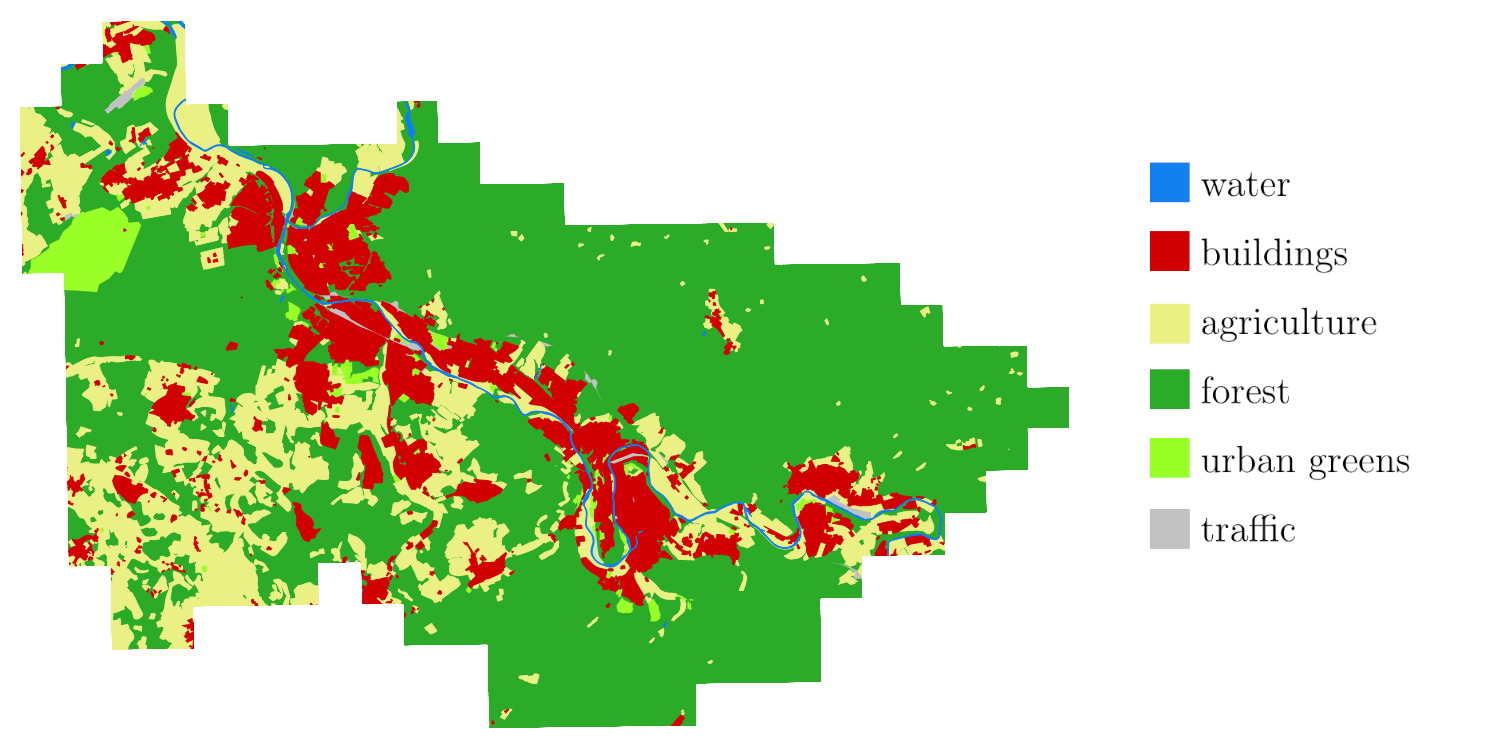
\includegraphics[width=\textwidth]{images/dop_label_all}
    \caption{The labels in the dataset}
    \label{fig:dop_label_all}
\end{figure}

\subsection{Export images for training}
\WIP{
for training, networks need fixed set of training/validation data. images and labels are prepared in database, but that does not work well for training. for efficient training process, dataset should be ready to use (like only read files and don't do any further processing). Very inefficient to export training batches live while training. it is better to export and save dataset in prepared batches, that can be fed directly into the network.

spatial image dimension are given by reference architectures. each architecture has different needs in regards to for example the input size of images and labels. But in general, all architectures need images with given resolution.

there is a general process to generate those images. create PostGIS geometry tiles to outline the training batches. then render those tiles with the DOP RGB bands to have input images. render it again with the segmentation info, to get the labels.

there is a python script to generate valid tiles that can be exported for training. basically it creates a bounding box for the region where data is available. inside that box, it creates all possible square tiles using the specified tile size. and last step is to remove all tiles that are not fully included in the region where data is available.

with all the tiles outlined, it is possible to generate images/label now. This can be done using the PostGIS raster bands and merging/intersecting them in a smart way. Still this would take a long time. It was found that this process is faster when using QGIS, an application to show/render geospatial data. it has a python API, allowing to run automatized exports. This is the way we go, rendering all tiles with image data and also all tiles with the segmentation info.

unfortunately, for rendering the segmentation info QGIS does interpolation for borders between segments. This is not what we want, because for the labels each pixel should clearly belong to one category. Thus, we have another script to correct the rendered labels. this just takes the interpolated pixels and assigns them to one of the adjacent categories in the label. After that, the images and labels are ready to use.
}

\begin{figure}
    \newcommand{\DopLabelImageWidth}{0.23\textwidth}
    \centering
    \hfill
    \begin{subfigure}{\DopLabelImageWidth}
        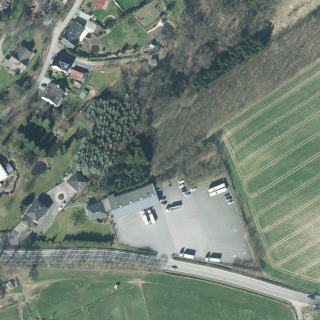
\includegraphics[width=\textwidth]{images/186_image}
    \end{subfigure}
    \hfill
    \begin{subfigure}{\DopLabelImageWidth}
        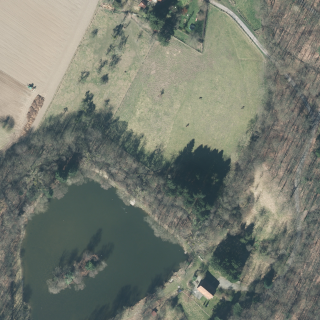
\includegraphics[width=\textwidth]{images/583_image}
    \end{subfigure}
    \hfill
    \begin{subfigure}{\DopLabelImageWidth}
        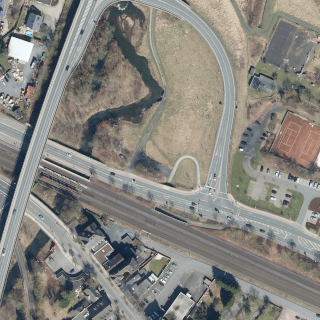
\includegraphics[width=\textwidth]{images/2281_image}
    \end{subfigure}
    \hfill
    \begin{subfigure}{\DopLabelImageWidth}
        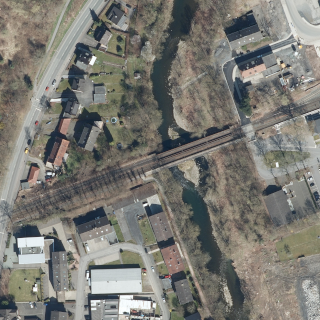
\includegraphics[width=\textwidth]{images/3589_image}
    \end{subfigure}
    \hfill

    \vspace{3mm}

    \hfill
    \begin{subfigure}{\DopLabelImageWidth}
        
\includegraphics[width=\textwidth]{images/186_label}
    \end{subfigure}
    \hfill
    \begin{subfigure}{\DopLabelImageWidth}
        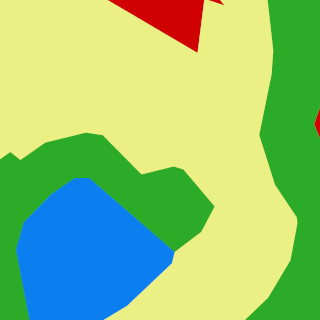
\includegraphics[width=\textwidth]{images/583_label}
    \end{subfigure}
    \hfill
    \begin{subfigure}{\DopLabelImageWidth}
        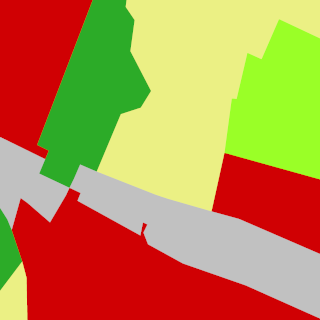
\includegraphics[width=\textwidth]{images/2281_label}
    \end{subfigure}
    \hfill
    \begin{subfigure}{\DopLabelImageWidth}
        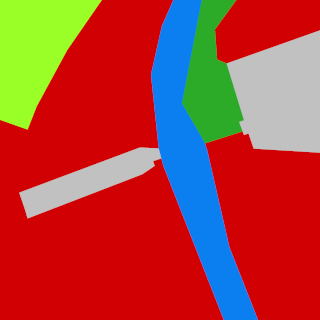
\includegraphics[width=\textwidth]{images/3589_label}
    \end{subfigure}
    \hfill

    \caption{Some image tiles with the respective labels}
    \label{fig:dop_with_labels}
\end{figure}

\subsection{Considerations about the dataset}
\WIP{
shapes in the labels are not super accurate. on macroscopic point of view, they cover all segments on large areas. but borders between segments are oftentimes poorly represented. meaning transition between forest and agriculture or coastal line along rivers modelled very roughly. to get really good training results one should preferably use pixel-perfect labels. for purpose of this thesis, where the goal is to identify suitable emergency landing areas, this might not be a big issue as we are looking for open wide areas and don't care to much about perfect borders. But anyway, keep it in mind during model training.
% TODO: show images/labels to support this argument

Another thing is distribution of segmentation classes in the dataset. table~\ref{tab:seg-breakdown} shows relative coverage of the area with the categories. you can see that around 65\% of the data set consist of forest. On the other hand the area of traffic and water combined is still under 1\%. In general, this is really bad for training DNNs. Will lead the network to predicting forest way more often than water/traffic. For optimal results the categories should be well balanced inside the training dataset. So this is also a point to consider later on.
% TODO: find a paper to support this argument
}

\subsection{Choose the test dataset}
\WIP{

}

\begin{table}[h]
\centering
\begin{tabular}{|l|r|r|r|r|r|}
\hline
\multicolumn{1}{|c|}{\textbf{segment}} &
  \multicolumn{1}{c|}{\textbf{total $m^2$}} &
  \multicolumn{1}{c|}{\textbf{total rel. $m^2$}} &
  \multicolumn{1}{c|}{\textbf{test $m^2$}} &
  \multicolumn{1}{c|}{\textbf{test rel. $m^2$}} &
  \multicolumn{1}{c|}{\textbf{test / total}} \\ \hline
forest       & 162,554,698 & 65.40\% & 17,430,019 & 61.63\% & 10.72\% \\ \hline
buildings    & 30,821,514  & 12.40\% & 3,827,202  & 13.53\% & 12.42\% \\ \hline
urban greens & 5,715,026   & 2.30\%  & 716,624    & 2.53\%  & 12.54\% \\ \hline
agriculture  & 47,331,698  & 19.04\% & 5,898,601  & 20.86\% & 12.46\% \\ \hline
water        & 1,344,467   & 0.54\%  & 273,114    & 0.97\%  & 20.31\% \\ \hline
traffic      & 788,878     & 0.32\%  & 135,977    & 0.48\%  & 17.24\% \\ \hline
\end{tabular}
\caption{Breakdown of segments}
\label{tab:seg-breakdown}
\end{table}

\newpage
